\documentclass[lettersize,journal]{IEEEtran}
\usepackage{amsmath,amsfonts}
\usepackage{algorithmic}
\usepackage{array}
\usepackage[caption=false,font=normalsize,labelfont=sf,textfont=sf]{subfig}
\usepackage{textcomp}
\usepackage{stfloats}
\usepackage{url}
\usepackage{verbatim}
\usepackage{graphicx}
\hyphenation{op-tical net-works semi-conduc-tor IEEE-Xplore}
\def\BibTeX{{\rm B\kern-.05em{\sc i\kern-.025em b}\kern-.08em
    T\kern-.1667em\lower.7ex\hbox{E}\kern-.125emX}}
\usepackage{balance}
\usepackage{booktabs}
\usepackage{bm}
\usepackage{bbm}
\usepackage{float}
\usepackage{hyperref}
\usepackage{dsfont}





\begin{document}
\title{Computer Vision\\ \vspace{.5em} 
\Large Multi-label Image Classification}
\author{Group 25 \\ \vspace{.2em} Riajul Islam, Andreas Calonius Kreth, Christine Midtgaard}



\maketitle

% Todo:
% [] Describe the multi-label classification problem and its challenges.

% [] Explain each method's theoretical background and mechanisms.

% [] Compare their approaches to the problem.

% [] Reproduce their models, train and evaluate them.

% [] Compare your results with those reported in the papers.

% [] Evaluate the feasibility and performance of each method.

\begin{abstract}
Abstract goes here.
\end{abstract}

\begin{IEEEkeywords}
Multi-label learning, deep learning, computer vision, multi-label
classification, deep learning for MLC. 

\end{IEEEkeywords}

% ======================== Introduction ========================

\section{Introduction}

% [] Introduce the multi-label image classification problem and its challenges.

% [] Mention the two methods you investigate.

% [] Explain that your aim is to reproduce the results and evaluate their performance on MS-COCO.

% [] Clarify that the methods are not compared directly, but evaluated independently against the reported baselines.


Multi-label classification is the supervised learning problem where an instance may be associated with multiple labels. Image classification is a computer vision task that requires assigning a label or multiple labels to an image. Single-label classification, or multi-class classification, refers to the problem where an image contains only one object to be identified. However, natural images usually contain multiple objects or concepts, highlighting the importance of multi-label classification \cite{ridnik2021mldecoderscalableversatileclassification}. 

In this project we investigate methods aimed to solve two common issues that arise when training a network that assigns multiple labels to an input image: (i) the general multi-label learning issue accurately identifying multiple objects in an image under class imbalance, representing the complexity of real-world images, and (ii) the scenario where the training data underwent sparse supervision.


\subsection{Problem Overview}

\paragraph{Label Correlation}
\paragraph{Class Imbalance}
\paragraph{Sparse Supervision}


\section{Related Work}
Multi-label learning is a well studied problem within computer vision \cite{mlsp}. 

% [] Provide a concise review of existing methods in multi-label classification.

% [] Include references to transformer-based methods (like Q2L), and weakly supervised learning methods (like MLSPL).

\paragraph{Loss Functions}

\paragraph{PU learning} 
Learning from positive and unlabeled data: a survey by Bekker and Davis \cite{Bekker_2020}.

Learning to Classify Texts Using Positive and Unlabeled Data by Li and Liu \cite{Li_2003}.

\paragraph{Partially Observed Labels}
% Learning a Deep ConvNet for Multi-label Classification with Partial Labels https://arxiv.org/pdf/1902.09720

\paragraph{Heuristics}
Heuristics can be used to reduce the required
annotation effort [34, 18], but this runs the risk of increasing
error in the labels \cite{mlsp}.

% ======================== Theoretical Background ========================
\section{Background}
This section describes relevant background theory related to the project and methods from MLSPL and Query2Label. Beginning with the definition of multi-label learning, followed by deep neural network architectures used to solve multi-label slassification tasks, and, finally, loss functions as they can handle challenges of label imbalance tasks.

\subsection{Multi-Label Learning}
Contrary to binary or multi-class classification where each instance is associated with only one label, multi-label classification allows assigning multiple labels to a single input \cite{mlsp}. Given $K$ categories, an input image $x\in \mathcal{X}$ is associated with a binary vector of labels $y=[y_1,...,y_K]$ from the label space $\mathcal{Y}=\{0,1\}^K$, where $y_k=1$ represents that $k$ is present in $x$ and $y_k=0$ otherwise. The goal is to create a model that outputs the probability of the presence of a category $p=[p_1,...,p_K]$ \cite{mlsp,Query2Label}.

\subsection{Convolutional Neural Networks (CNNs)}
In the field of computer vision, Convolutional Neural Networks (CNNs) have been a dominant approach for image analysis tasks since their introduction \cite{lecun95}. CNNs are designed to recognize patterns in images by applying local filters through convolutional layers, preserving the two dimensional input of an image \cite{zhang2023dive}. CNNs consist of three main types of layers: convolutional layers, pooling layers, and a Fully Connected (FC) layer \cite{asawaCS231n}. Convolutional layers extract spatial features through learnable filters, pooling layers reduce dimensionality and summarise information, while the fully connected layer at the end interpret the features to perform the classification.

\subsection{Transformer Architectures}
Transformers, introduced by Vaswani et al. \cite{vaswani2023attentionneed}, are a type of neural network architecture initially developed to model long-range dependencies in sequence data. They achieve this using attention and self-attention mechanisms, which enables the model to have a long-term memory of inputs, and dynamically weigh the importance of each element in the input sequence. Originally, transformer-based models was mainly delevoped for natural language processing tasks, but the introduction of the Vision Transformer (ViT) by Dosovitskiy et al. \cite{dosovitskiy2021imageworth16x16words}, transformers have been widely used for computer vision tasks. 

\paragraph{Architecture}
The original transformer consists of an encoder-decoder structure. Both encoder and decoder are made of a stack of identical layers, where encoder layers contain a multi-head self-attention mechanism followed by a position-wise feed-forward network. In addition, decoder layers consists of an encoder-decoder attention layer. 

The transfomer encoder is of interest, as the authors of \cite{Query2Label} use them to extract features and automatically learn label embedding, as described in section \ref{sec:q2l_method}.

\paragraph{Attention}
The core principle of the transformer architecture is the attention mechanism, which allows the model to attend to all posistions in an input sequence when processing each element. Thus alloowing the model to weigh the relevance of different posistions in a sequence. Given a query and a set of key-value pairs, the attention function computes a weighted sum of the values, where the weights are determined by similarities between the query and the keys.

\paragraph{Self-Attention}
The transformer model uses self-attention by relating every element in the input sequence to every other element. The attention function is a function that maps a query and a set of key-value pairs to an output. The scaled dot-product self-attention is defined as:

\begin{equation}
    \text{Attention}(Q,K,V) = \text{softmax}\left(\frac{QK^T}{\sqrt{d_k}}\right)V
\end{equation}

\noindent where $Q$, $K$, $V$, are the query, key, and value vectors, and $d_k$ is the dimension of the key vectors and serves as a scaling factor \cite{vaswani2023attentionneed}. 

\paragraph{Multi-Head Attention}
The transformer applies multiple attention functions in parallel, allowing the model to attend to information from different parts of the sequence. The embedding is split into multiple heads, perform attention for each, and then concatenate them back together, defined as:

\begin{equation}
    \text{MultiHead}(Q,K,V) = \text{Concat}(\text{head}_1, ..., \text{head}_h)W^O
\end{equation}
    
\noindent where each head is computed as:

\begin{equation}
    \text{head}_i = \text{Attention}(QW^Q_i, KW^K_i, VW^V_i)
\end{equation}

\noindent with projection matrices $W_i^Q$, $W_i^K$, $W_i^V$, and $W_i^O$.

\paragraph{Cross-Attention}
Contrary to self-attention, where queries, keys, and values are generated from the same input, cross-attention is a mechanisn where queries come from one source, and the keys and values come fron another. This mechanism allows the model to relate elements from one input to relevant parts of another input. The authours of Query2Label \cite{Query2Label} make use of this mechanism, where label embeddings (queries) attend to spatial image features (key-value pairs).

\paragraph{Feed-Forward Networks and Positional Encoding}
Each layer in the Transformer also includes a fully connected feed-forward network applied to each position. To compensate for the lack of order in the input sequence, sinusoidal positional encodings are added to the input embeddings. These encodings allow the model to distinguish the order of elements in the sequence using functions of varying frequencies.

\paragraph{Vision Transformers (ViTs)}
The Vision Transformer (ViT), introduced by Dosovitskiy et al. \cite{dosovitskiy2021imageworth16x16words}, is a model for image classification that leverages the transformer architecture: the self-attention mechanism of transformers that allows the model to selectively weigh the significance of each part of the input, and positional embeddings that represent the order of tokens in a sequence. In ViTs, images are represented as sequences, where the label function as a learnable token for classification. The input image is divided into a sequence of patches that are flattened and linearly embedded into a vector. The spatial information is preserved by adding positional encodings to the embeddings. The resulting sequence is fed into a transformer decoder identical to that introduced in \cite{vaswani2023attentionneed} to model global relations for classification.

\subsection{Loss Functions}
Loss functions are a fundamental component in deep learning as they serve as a measure of how much the model predictions deviate from the ground truth, guiding optimization of the network \cite{zhang2023dive}. The goal of optimization is to minimize the loss. In the context of multi-label learning, each instance can belong to multiple classes simumtaneously, and selecting an appropriate loss function is crucial. This section aims to decribe different loss functions employed in multi-label classification, and how they can be used to solve common issues in multi-label learning.

\paragraph{Binary Cross-Entropy (BCE)}
Due to its effectiveness in handling binary decisions for each class, a common choice of loss function for multi-label classification is the The Binary Cross-Entropy (BCE) loss \cite{mlsp,durand2019learningdeepconvnetmultilabel,nayan2024binary}. In binary classification, the goal is to classify data as either positive or negative, represented as 0 or 1. The output of the model is a probability score between 0 and 1, indicating the probability of the input belonging to the positive class \cite{nayan2024binary}.

The BCE loss for multi-label classification is given by:

\begin{equation}
\begin{aligned}
\mathcal{L}_{\text{BCE}} = -\frac{1}{K} \sum_{i=1}^{K} \bigl[ &y_i\log(p_i) \\
+ &(1-y_i)\log(1 - p_i) \bigr]
\end{aligned}
\end{equation}

\noindent where $K$ is the number of categories, $y_i\in[0,1]$ is the binary label, and $p_i$ is the predicted probability.

Due is its popularity in multi-class classification the BCE loss is used as a benchmark for model performance in \cite{mlsp}. However, BCE loss can be sensitive to class imbalance, where some classes appear more often than others. In this case, the model tend to focus on the majority class and perform poorly on the minority class. 

\paragraph{Loss Functions for the Partially Observed Labels Setting}
BCE assumes that each training example indicates the presence or absence of each class, e.i. the example is fully observable. In real-world multi-label datasets, it is often infeasible to annotate all relevant labels for each image, resulting in only partially observed labels. In the case where labels are only partially observed, the assumption of full negative labeling in BCE can lead to false negatives during training, degrading model performance \cite{mlsp}. 

To address this issue, several loss functions have been proposed to handle partial supervision \cite{mlsp}. In this project, we explore the case of minimal supervision: the single positive label setting, where only one relevant class label is observed per image and the rest are unannotated. The authors of \cite{mlsp} propose Expected Positive Regularization (EPR) and Regularized Online Label Estimation (ROLE) as solutions, described in the following.

\paragraph{Expected Positive Regularization (EPR)}
Assuming that unobserved labels are negative leads to the BCE loss for the positive only case:

\begin{equation}
    \mathcal{L}_{BCE}^+(\mathbf{f}_n,\mathbf{z}_n) = - \sum_{i=1}^{L}\mathds{1}_{[z_{ni}=1]}\log(f_{ni})
\end{equation}

However, this predicts all labels as positive. The solution to this is the introduction of a regularization term that contains a domain knowledge. They define a scalar $k$, which is the expected number of positives per image, and an estimated average number of predicted positves $\hat{k}(\mathbf{F}_B)$ from batch predictions, where $\mathbf{F}_B = [f_{ni}]_{n\in B,i\in\{1,...,L\}}$ is defined to be the predictions $f_{ni}\in[0,1]$ for every image in a batch $B\subset \{1,...,N\}$. A regularization term at batch level is introduced to penalize deviations from $k$:

\begin{equation}
    R_k(\mathbf{F}_B) = \left(\frac{\hat{k}(\mathbf{F}_B)-k}{L}\right)^2
\end{equation}

\noindent The overall loss is:

\begin{equation}
    \mathcal{L}_{EPR}(\mathbf{F}_B,\mathbf{Z}_B) = \frac{1}{|B|}\sum_{n\in B}\mathcal{L}_{BCE}^+(\mathbf{f}_n,\mathbf{z}_n)+\lambda R_k(\mathbf{F}_B)\text{,}
\end{equation}

where $\lambda$ is a hyperparameter.

% \begin{equation}
%     k=\mathbb{E}_{(\mathbf{x},\mathbf{y})\sim p_{\text{data}(\mathbf{x},\mathbf{y})}}\sum_{i=1}^{L}\mathds{1}_{[y_i=1]}
% \end{equation}

% \noindent where $\mathds{1}[\cdot]$ denotes the indicator function, i.e. $\mathds{1}_{[zni=1]} = 1$ if $z_{ni} = 1$, and $0$ otherwise. $k$ can either be estimated from data or treated as a hyperparameter. A matrix $\mathbf{F}_B = [f_{ni}]_{n\in B,i\in\{1,...,L\}}$ is defined to be the predictions $f_{ni}\in[0,1]$ for every image in a batch $B\subset \{1,...,N\}$. The batch predictions a used to compute 

% \begin{equation}
%     \hat{k}(\mathbf{F}_B) = \frac{\sum_{n\in B}\sum_{i=1}^{L}\mathbf{f}_{ni}}{|B|}\text{.}
% \end{equation}

% Let $\mathbf{Y}_B = [y_{ni}]_{n\in B,i\in\{1,...,L\}}$ be the matrix of true labels, where perfect predictions would yield $\mathbf{F}_B=\mathbf{Y}_B$. In this case, $\mathbb{E}[\hat{k}(\mathbf{F}_B)]=\mathbb{E}[\hat{k}(\mathbf{Y}_B)]$, naturally leading to $\hat{k}=k$. The EPR loss introduces a regularization term $R_k(\mathbf{F}_B)$ that encourages $\hat{k}$ to be as close to $k$ as possible, penalizing negatives, leading to the EPR loss defined as followed:



\paragraph{Regularized Online Label Estimation (ROLE)}
The authors of \cite{mlsp} report that $\mathcal{L}_{EPR}$ does not yield satisfactory results, and thus propose a combination of $\mathcal{L}_{EPR}$ and a label estimator module that maintains online estimates of the missing labels during training, called Regularized Online Label Estimation (ROLE). This method jointly trains the image classifier and a label estimator subject to constraints imposed by $\mathcal{L}_{EPR}$. This maintains soft estimates of the full label vector during training, resulting in ROLE assuming unobserved labels to have a probability between 1 and 0. For a batch $B$, let $\mathbf{\tilde{Y}}\in[0,1]^{N\times L}$ represent the estimated labels, and $\mathbf{F}\in[0,1]^{N\times L}$ represent the matrix of classifier predictions. The goal is to jointly train the label estimator $g(\cdot;\phi)$ and the image classifier $f(\cdot;\theta)$. An intermediate loss is defined as:

\begin{equation}
    \label{eq:mlsp_11}
    \begin{aligned}
        \mathcal{L}'(\mathbf{F}_B,\tilde{\mathbf{Y}}_B) &= \frac{1}{|B|}\sum_{n\in B} \mathcal{L}_{BCE}(\mathbf{f}_n,\text{sg}(\tilde{\mathbf{y}}_n)) \\
        &+ \mathcal{L}_{EPR}(\mathbf{F}_B,\mathbf{Z}_B)\text{,}
    \end{aligned}
\end{equation}

\noindent where $\text{sg}$ is a stop-gradient. This loss is used to update $\theta$ while keeping $\phi$ fixed. By switching the arguments in Eq.~\ref{eq:mlsp_11}, $\phi$ is updated while keeping $\theta$ fixed. This leads to the final ROLE loss, given by:

\begin{equation}
    \mathcal{L}_{ROLE}(\mathbf{F}_B, \mathbf{\tilde{Y}}_B) = \frac{\mathcal{L}'(\mathbf{F}_B)|\mathbf{\tilde{Y}}+\mathcal{L}'(\mathbf{\tilde{Y}}|\mathbf{F}_B)}{2}
\end{equation}

\noindent where both $\mathbf{F}_B$ and $\tilde{\mathbf{Y}}_B$ are updated simultaneously.



% ======================== Methodology ========================

\section{Method}
% Focus Methodology on the rationale for choosing these methods, how the operationalized their training, and any adaptations made for reproduction.

In real-world datasets, obtaining full label annotations is practiaclly impossible.
This project focuses on finding solutions to the multi-label learning problems:
\begin{itemize} 
    \item  The challenge of multi-label learning in scenarios where only a single positive label per image is available durin training (MLSPL).
    \item Label imbalance (Query2Label).
    \item Feature localization (Query2Label).
\end{itemize}

\subsection{Overview of Approach}
A brief description of what we did to solve the multi-label classification problem. 



\subsection{Query2Label: A Simple Transformer Way to Multi-Label Classification}
\label{sec:q2l_method}
Query2Label: A Simple Transformer Way to Multi-Label Classification (Query2Label) by Liu et al. \cite{Query2Label} is a two-stage framework for multi-label classification. It uses transformer decoders to extract features with multi-head attentions focusing on different parts of an object category and learn label embeddings from data automatically.

\subsection{Multi-Label Learning from Single Positive Labels}
MLSPL's solution to a sparsely annotated training dataset is twofold: first, they develop a training methodology using datasets where annotators have only provided a single confirmed positive label per image, with no confirmed negatives. Second, they extend existing multi-label loss functions to handle this challenging scenario and introduce novel variants to constrain the expected number of positive labels.

\begin{figure}[h]
    \centering
    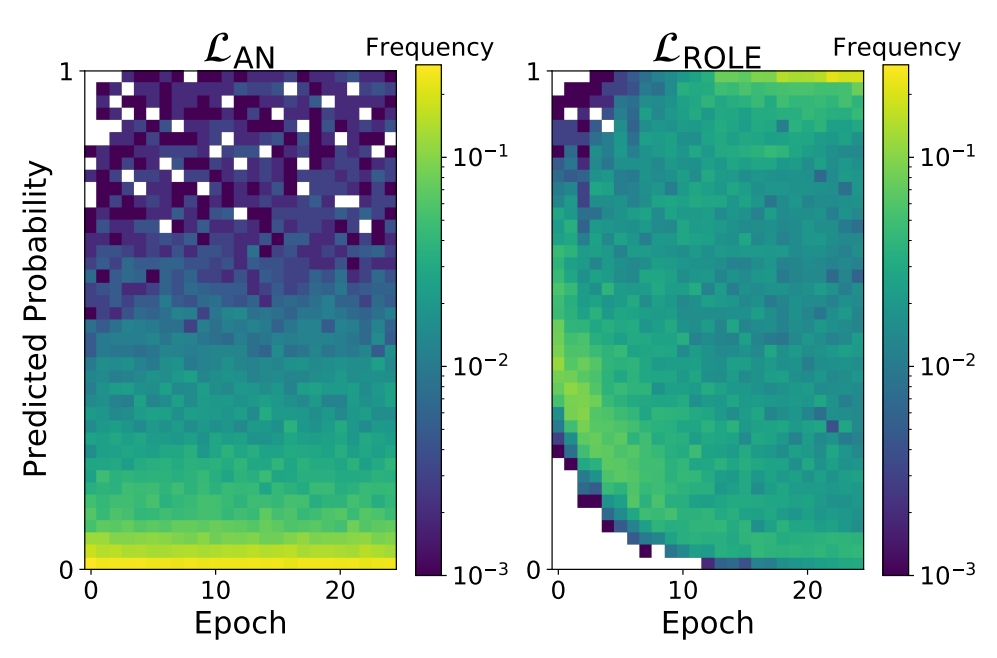
\includegraphics[width=.8\linewidth]{images/mlsp_fig2.png}
    \caption{Figure 2 in MLSPL \cite{mlsp}. The distribution of predicted probabilities for unobserved positives when training with a single positive per image for COCO.}
    \label{fig:mlsp_fig2}
\end{figure}


% ======================== Experimental Setup  ========================

\begin{table*}[t]
    \small
    \caption{Comparison of mAP results from our experiments and the reported results on Query2Label on the MS-COCO 2014 Dataset.}
    \label{tab:q2l_map_comparison}
    \centering
    \begin{tabular}{l l l c c}
    \toprule
    \textbf{Method} & \textbf{Backbone} & \textbf{Resolution} & \textbf{mAP(Ours)} & \textbf{mAP (Paper)} \\
    \midrule
    Q2L-R101     & ResNet-101     & $448\times448$ & 84.9 & 84.9 \\
    Q2L-R101     & ResNet-101     & $576\times576$ & 86.5 & 86.5 \\
    Q2L-TresL    & TResNetL       & $448\times448$ & 87.3 & 87.3 \\
    Q2L-Tres     & TResNetL(22k)  & $448\times448$ & 89.2 & 89.2 \\
    Q2L-SwinL    & Swin-L(22k)    & $384\times384$ & 90.5 & 90.5 \\
    Q2L-CvT      & CvT-w24(22k)   & $384\times384$ & 91.3 & 91.3 \\
    \bottomrule
    \end{tabular}
\end{table*}

\section{Experiments}
All experiments were conducted on a cluster with access to two NVIDIA GeForce RTX 3060 GPU (12 GB VRAM). The cluster was equipped with Ubuntu 22.04.5 LTS.

\subsection{Dataset}
The MS-COCO 2014 \cite{coco14} dataset is used as a benchmark for evaluation both Query2Label and MLSPL. MS-COCO (Microsoft Common Objects in Context) is a large-scale dataset commonly used for object detection, segmentation, and multi-label image classification. COCO consists of 82,081 training images and 80 classes, and a validation set of 40,137 images.

\begin{figure}[t]
    \centering
    \includegraphics[width=.8\linewidth]{images/coco_grid.png}
    \caption{Examples from the MS-COCO 2014 training set, resized to $448 \times 448$ pixels.}
    \label{fig:coco-examples}
\end{figure}

\subsection{Evaluation Metrics}
To asses model performance, we adopt mean Average Precision (mAP), a standard metric widely reported in multi-label classification tasks as it is used to analyze the performance on object detection and segmentation. Both Query2Label and MLSPL report results in terms of mAP. 

\subsection{Query2Label}
All Query2Label experiments were conducted using Python 3.7.3 with PyTorch 1.9.0 and Torchvision 0.10.0, compiled with CUDA 11.1. Due to compatibility issues with the \texttt{inplace\_abn} dependency required by TResNet backbones, we rebuilt the extension from source using commit \texttt{938ffd2} to ensure compatibility with our environment.

Additionally, we encountered a missing dependency for RandAugment, which was not included in the original repository. To address this, we manually added the augmentations.py file from the pytorch-randaugment implementation\footnote{\url{https://github.com/ildoonet/pytorch-randaugment}} and modified the import in get\_dataset.py to use a local version: from .augmentations import RandAugment. We also replaced the default RandAugment() instantiation with RandAugment(n=2, m=9) to explicitly set the parameters. While a similar implementation exists in the torchvision.transforms module\footnote{\url{https://pytorch.org/vision/main/generated/torchvision.transforms.RandAugment.html}}, it is incompatible with the version of torchvision used in this project.

\paragraph{Data preparation}
While the original work includes experiments on five datasets, our reproduction is limited to the MS-COCO 2014 dataset. The model was evaluated on the MS-COCO 2014 dataset. All images were resized to match the input resolution required by each respective backbone. Label annotations for each image were preserved in their multi-label format.

\paragraph{Training}
Attempts to train Query2Label with the CvT-w24 backbone failed due to memory limitations of the available 12GB GPUs. However, due to time constraints, we did not replicate the original training procedure using our own setup, and only tested if training was possible with the limited memory availability, and instead, we relied on the publicly released pretrained models provided by the authors. The Query2Label framework was evaluated using four backbone configurations: ResNet-101 at resolutions of $448\times448$ and $576\times576$, as well as Swin-L(22k) and CvT-w24(22k) at $384\times384$, both pretrained on the ImageNet-22k \cite{imagenet} dataset. These models were originally trained on the MS-COCO 2014 training set and evaluated in our experiments on the MS-COCO 2014 validation set. We used a batch size of 16 and made no further modifications or fine-tuning.

We tested training the Query2Label model from scratch using the ResNet-101 backbone. Distributed training was enabled to leverage both GPUs. Training was conducted with a batch size of 8, chosen to fit within the memory constraints of the GPUs. The model was optimized using AdamW with a learning rate of $10^{-4}$, weight decay of $10^{-2}$, and trained for 80 epochs with early stopping enabled. Data augmentation included random cutout with one hole and a cut factor of 0.5. Four data loading workers were used per process. No modifications were made to the original model architecture or loss design.


\subsection{Multi-Label Learning from Single Positive Labels}
The original implementation was developed with older library versions, specifically PyTorch 1.7.0+cu110, and Torchvision 0.8.1+cu110. In contrast, our reproduction was conducted using PyTorch 2.2.1+cu121, and Torchvision 0.17.1+cu121. The original implementation had unknown versions of Python and CUDA, whereas our experiments were conducted using python 3.11.8 and CUDA 12.4. Despite keeping the code unchanged, and using the original random seed, differences in default behavior between library versions may cause deviations in results. Nevertheless, all code ran without modification, and we verified that training and evaluation completed successfully.

Although two GPUs were available on the system, only a single GPU was utilized during training to maintain consistency and reproducibility of the results.

\paragraph{Data preparation}
While the original work includes experiments on four datasets, our reproduction is limited to the MS-COCO 2014 dataset. The COCO dataset was converted to a single-positive label format to simulate a weakly supervised setting. Following Cole et al.~\cite{mlsp}, this was done by starting with the fully annotated multi-label dataset and corrupting it by discarding all but one randomly selected positive label per image. Importantly, the same selected label is consistently used throughout training to ensure fair comparisons across methods. Additionally, 20\% of the training data was set aside for validation. Both the validation and test sets remain fully labeled.

To prepare the data, we followed the authors' instructions: first, the standard COCO 2014 training and validation images and annotations were downloaded. Next, we obtained the pre-extracted features provided by the authors. Finally, the \texttt{format\_coco.py} script was used to produce uniformly formatted image lists and corresponding labels.


\paragraph{Training}
Results are reported on two training scenarios: (i) linear classification on fixed features and (ii) end-to-end fine-tuning. For each method, a hyperparameter search was conducted, and results are reported for the configuration achieving the best mean average precision (mAP) on the validation set.

In replicating the experiments, we conducted a similar hyperparameter search, considering learning rates  $\{1e-2, 1e-3, 1e-4, 1e-5\}$ and batch sizes ${8, 16}$. The linear classifier was trained for 25 epochs, and the fine-tuning phase for 10 epochs. The validation set used was the clean variant, meaning it was fully labeled.

\paragraph{Selected Hyperparameters}
The final results reported for MS-COCO were obtained using the hyperparameters that achieved the highest validation mAP during the search. For the linear classifier, we used a batch size of 16 and a learning rate of 0.001. For the fine-tuned ResNet-50 model, the learning rate was set to 0.00001, with the same batch size of 16.

% ======================== Results and Discussion ========================

\section{Results and Discussion}
\label{sec:results}
This section compares results from the experiments to the those of the papers. Discuss why they might not be the same, or describe the similarities. Discuss whether the methods are able to solve the problems.


\subsection{Results from Query2Label}
The results from our experiments are compared to those of the paper in table \ref{tab:q2l_map_comparison}. 



\subsection{Results from Multi-Label Learning from Single Positive Labels}
The results from our experiments are compared to those of the paper in table \ref{tab:MLSPL_map_comparison}. 

\begin{table}[H]
    \small
    \caption{Comparison of mAP results from our experiments and the reported results on Multi-Label Learning from Single Positive Labels on the MS-COCO 2014 Dataset.}
    \label{tab:MLSPL_map_comparison}
    \centering
    \begin{tabular}{l l c c}
    \toprule
    \textbf{Loss} & \textbf{Method} & \textbf{mAP(Ours)} & \textbf{mAP (Paper)} \\
    \midrule
    $\mathcal{L}_{ROLE}$ & Linear & 66.3 & 66.3 \\
    $\mathcal{L}_{ROLE}$ & Fine-Tuned & 66.9 & 66.3 \\
    \bottomrule
    \end{tabular}
\end{table}


% ======================== Conclusion ========================

\section{Conclusion}

Conclusion here.
% [] Summarize findings for each method.

% [] Mention if the results reproduced align with the papers.

% [] Suggest future directions or improvements.


\bibliographystyle{IEEEtran}
\bibliography{references}




\end{document}


